\documentclass{article}

\usepackage[english]{babel}
\usepackage[utf8]{inputenc}
\usepackage{amsmath,amssymb}
\usepackage{parskip}
\usepackage{graphicx}
\usepackage{listings}
\usepackage{subfig}
\usepackage{float}
\lstset{
    numbers=left, 
    numberstyle= \tiny, 
    keywordstyle= \color{ blue!70},
    commentstyle= \color{red!50!green!50!blue!50}, 
    frame=shadowbox, % 阴影效果
    rulesepcolor= \color{ red!20!green!20!blue!20} ,
    escapeinside=``, % 英文分号中可写入中文
    xleftmargin=2em,xrightmargin=2em, aboveskip=1em,
    framexleftmargin=2em,
    breaklines=true,
    language=R
} 

% Margins
\usepackage[top=2.5cm, left=3cm, right=3cm, bottom=4.0cm]{geometry}
% Colour table cells
\usepackage[table]{xcolor}

% Get larger line spacing in table
\newcommand{\tablespace}{\\[1.25mm]}
\newcommand\Tstrut{\rule{0pt}{2.6ex}}         % = `top' strut
\newcommand\tstrut{\rule{0pt}{2.0ex}}         % = `top' strut
\newcommand\Bstrut{\rule[-0.9ex]{0pt}{0pt}}   % = `bottom' strut

%%%%%%%%%%%%%%%%%
%     Title     %
%%%%%%%%%%%%%%%%%
\title{CSCI946 Assignment}
\author{Yao Xiao \\ SID 2019180015}
\date{\today}

\begin{document}
\maketitle

%%%%%%%%%%%%%%%%%
%   Problem 1   %
%%%%%%%%%%%%%%%%%
\section{Task 1: Hypothesis Testing}
\textbf{Null hypothesis:}

The approach1 and approach2 do not effectively improve student learning performance.

\textbf{Alternative hypothesis:}

The two new learning approaches do effectively improve student learning performance.

First, we should divide the datasets into 3 parts
\begin{lstlisting}

> dataframe <- read.csv("A1_performance_test.csv")
> app1 <- dataframe[dataframe$approach=="approach1",]$performance
> app2 <- dataframe[dataframe$approach=="approach2",]$performance
> appNo <- dataframe[dataframe$approach=="no_approach",]$performance
> summary(app1)
   Min. 1st Qu.  Median    Mean 3rd Qu.    Max. 
 -1.073  54.815  74.100  77.345  95.648 155.282 
> summary(app2)
   Min. 1st Qu.  Median    Mean 3rd Qu.    Max. 
  14.97   63.08   82.48   83.30  102.14  161.37 
> summary(appNo)
   Min. 1st Qu.  Median    Mean 3rd Qu.    Max. 
 -23.39   19.03   38.88   40.94   62.90  119.99 

> t.test(app1,appNo,var.equal = TRUE)

#	Two Sample t-test

# data:  app1 and appNo
# t = 11.93, df = 379, p-value < 2.2e-16
# alternative hypothesis: true difference in means is not equal to 0
# 95 percent confidence interval:
#  30.40739 42.40905
# sample estimates:
# mean of x mean of y 
# 77.34459  40.93637
> qt(p=0.05/2, df=379, lower.tail= FALSE)
# [1] 1.966243
\end{lstlisting}

We can see that $|1-11.93| > 1.97$, so the original hypthsis will be denied.

\begin{lstlisting}
> t.test(app2,appNo,var.equal = TRUE)

#  	Two Sample t-test

# data:  app2 and appNo
# t = 14.021, df = 401, p-value < 2.2e-16
# alternative hypothesis: true difference in means is not equal to 0
# 95 percent confidence interval:
#  36.42716 48.30779
# sample estimates:
# mean of x mean of y 
#  83.30384  40.93637 

> qt(p=0.05/2, df=401, lower.tail= FALSE)
# [1] 1.965897
\end{lstlisting}

We can see that $|1-14.021| > 1.966$, so the original hypthsis will be denied.

For the approach 1\&2:
\begin{lstlisting}
> t.test(app1,app2,var.equal = TRUE)

# 	Two Sample t-test

# data:  app1 and app2
# t = -1.9988, df = 414, p-value = 0.04629
# alternative hypothesis: true difference in means is not equal to 0
# 95 percent confidence interval:
#  -11.81998428  -0.09851884
# sample estimates:
# mean of x mean of y 
#  77.34459  83.30384 

> qt(p=0.05/2, df=414, lower.tail= FALSE)
# [1] 1.965711
\end{lstlisting}

We can see that $|1-1.9988| = 0.9988 < 1.9657$, the original hypothesis will not be denied.

\textbf{Conclusion:}

The two new learning approaches do effectively improve student learning performance.
In terms of improving students’ learning performance, there is no significant difference between approach1 and approach2.

\textbf{Souce Code:}
\begin{lstlisting}
dataframe <- read.csv("A1_performance_test.csv")
app1 <- dataframe[dataframe$approach=="approach1",]$performance
app2 <- dataframe[dataframe$approach=="approach2",]$performance
appNo <- dataframe[dataframe$approach=="no_approach",]$performance

summary(app1)
summary(app2)
summary(appNo)

t.test(app1,appNo,var.equal = TRUE)
qt(p=0.05/2, df=379, lower.tail= FALSE)

t.test(app2,appNo,var.equal = TRUE)
qt(p=0.05/2, df=401, lower.tail= FALSE)

t.test(app1,app2,var.equal = TRUE)
qt(p=0.05/2, df=414, lower.tail= FALSE)

\end{lstlisting}

\section{Task 2: Clustering}
\subsection{Answer 1}
The Iris dataset has 5 attributes: Sepal.Length, Sepal.Width, Petal.Length, Petal.Width, Species.
And the dataset has 150 datas and each data belongs to one of 3 species(setosa, versicolor, virginica),
for the species, it uses length and width of flower's sepal and petal to describe.

\begin{figure}[H]
    \subfloat{
        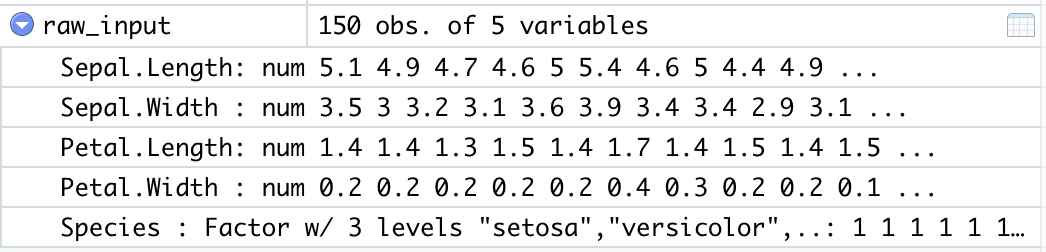
\includegraphics[width=1\textwidth]{Fig1}}\\
    \subfloat{
        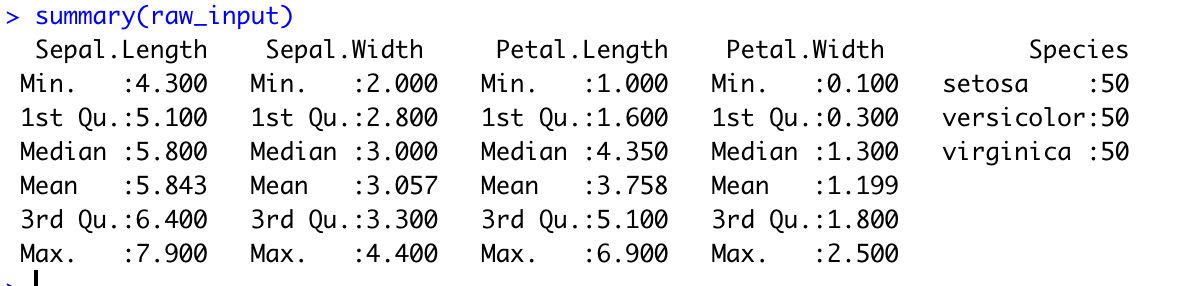
\includegraphics[width=1\textwidth]{Fig2}
    }
\end{figure}

\subsection{Answer 2}
\begin{figure}[H]
    \caption{Iris Dataset}
    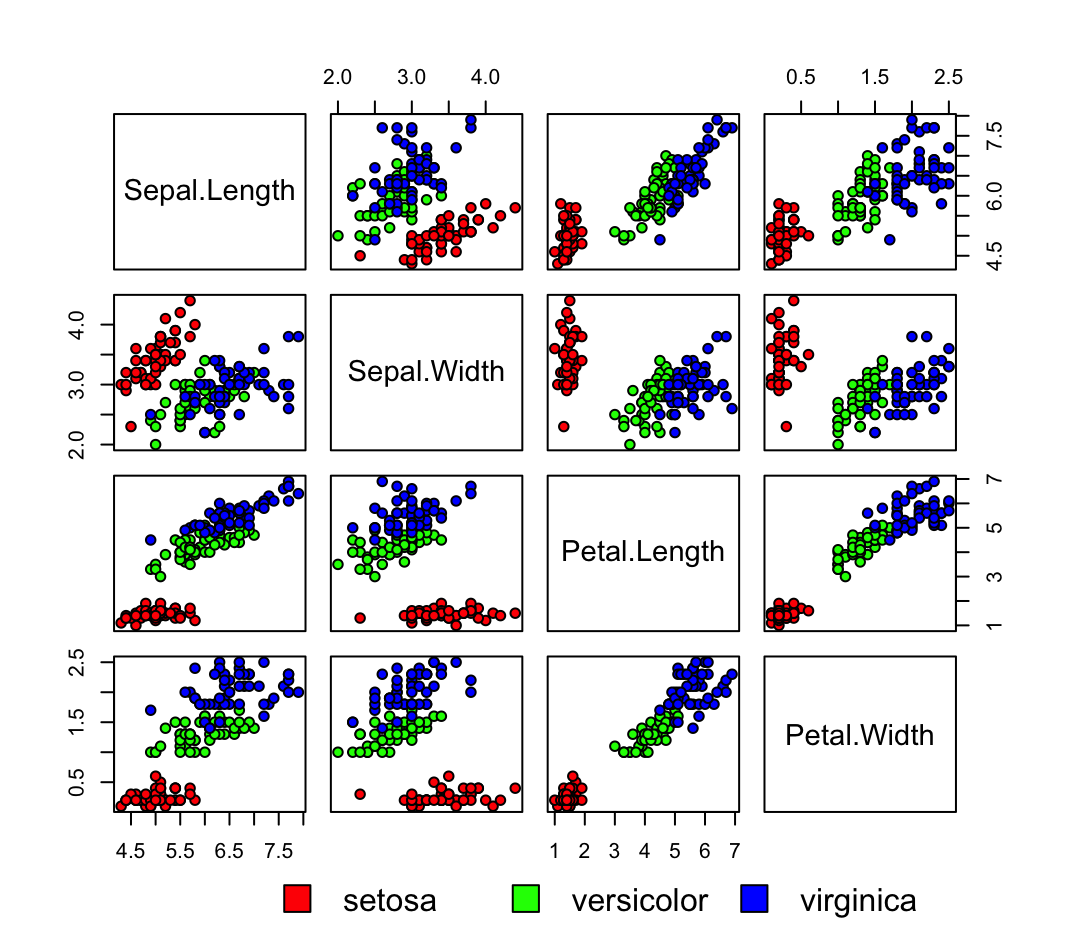
\includegraphics[width=1\textwidth]{Fig3}
\end{figure}

\subsection{Answer 3}
We should first remove the species attribute, and use the k-means algorithm to calculate the clustering k from 1 to 15, and calculate wss for each k value.

\begin{figure}[H]
    \caption{WSS of k value}
    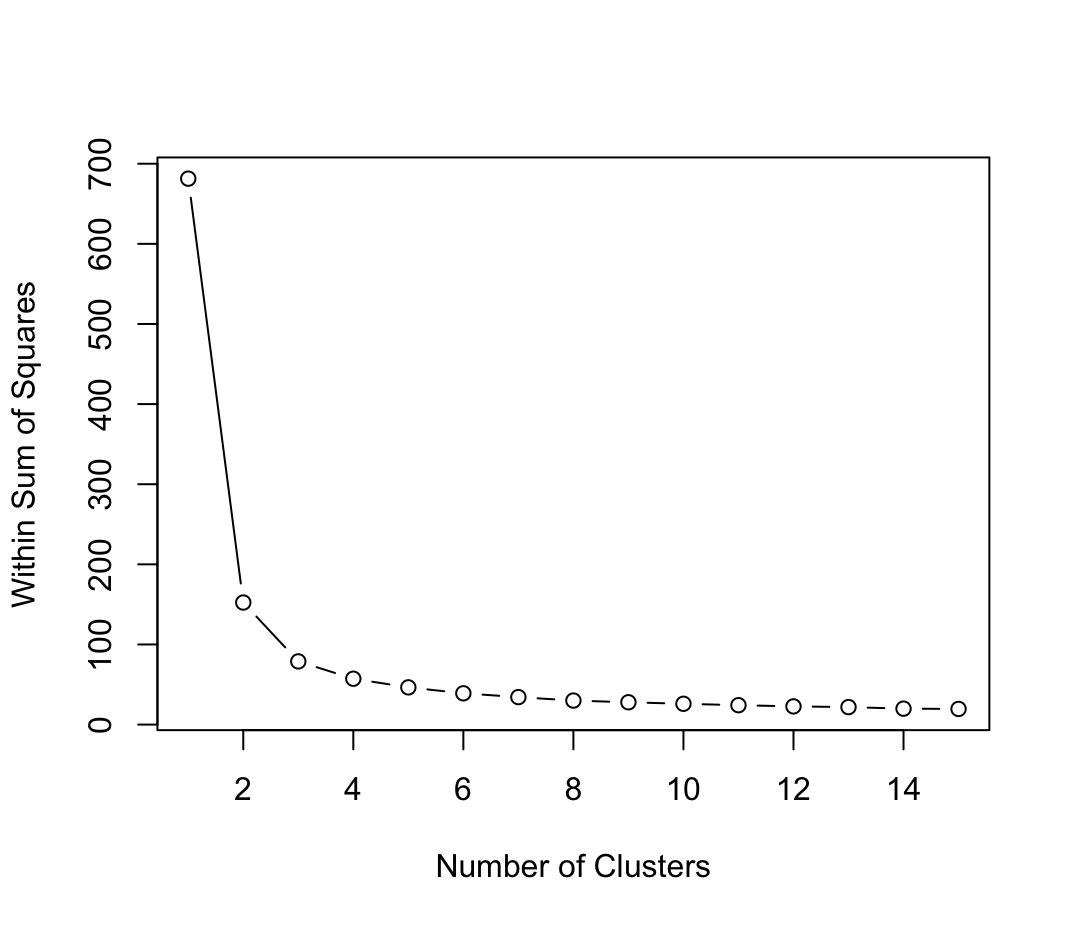
\includegraphics[width=1\textwidth]{Fig4}
\end{figure}

We can find when k > 3 from the figure 2, the trend of wss becomes linear.
Therefore, the k-means analysis should select k = 3.

\begin{lstlisting}
> km = kmeans(kmdata,3)
> km
# K-means clustering with 3 clusters of sizes 62, 50, 38

# Cluster means:
#   Sepal.Length Sepal.Width Petal.Length Petal.Width
# 1     5.901613    2.748387     4.393548    1.433871
# 2     5.006000    3.428000     1.462000    0.246000
# 3     6.850000    3.073684     5.742105    2.071053

# Clustering vector:
#  [1] 2 2 2 2 2 2 2 2 2 2 2 2 2 2 2 2 2 2 2 2 2 2 2 2 2 2 2 2 2 2 2 2 2 2 2 2 2 2
#  [39] 2 2 2 2 2 2 2 2 2 2 2 2 1 1 3 1 1 1 1 1 1 1 1 1 1 1 1 1 1 1 1 1 1 1 1 1 1 1
#  [77] 1 3 1 1 1 1 1 1 1 1 1 1 1 1 1 1 1 1 1 1 1 1 1 1 3 1 3 3 3 3 1 3 3 3 3 3 3 1
# [115] 1 3 3 3 3 1 3 1 3 1 3 3 1 1 3 3 3 3 3 1 3 3 3 3 1 3 3 3 1 3 3 3 1 3 3 1

# Within cluster sum of squares by cluster:
# [1] 39.82097 15.15100 23.87947
#  (between_SS / total_SS =  88.4 %)

# Available components:

# [1] "cluster"      "centers"      "totss"        "withinss"     "tot.withinss"
# [6] "betweenss"    "size"         "iter"         "ifault"      

> str(km)
# List of 9
#  $ cluster     : int [1:150] 2 2 2 2 2 2 2 2 2 2 ...
#  $ centers     : num [1:3, 1:4] 5.9 5.01 6.85 2.75 3.43 ...
#   ..- attr(*, "dimnames")=List of 2
#   .. ..$ : chr [1:3] "1" "2" "3"
#  .. ..$ : chr [1:4] "Sepal.Length" "Sepal.Width" "Petal.Length" "Petal.Width"
#  $ totss       : num 681
#  $ withinss    : num [1:3] 39.8 15.2 23.9
#  $ tot.withinss: num 78.9
#  $ betweenss   : num 603
#  $ size        : int [1:3] 62 50 38
#  $ iter        : int 2
#  $ ifault      : int 0
#  - attr(*, "class")= chr "kmeans"

> table(iris$Species,km$cluster)
            
#               1  2  3
#   setosa      0 50  0
#   versicolor 48  0  2
#   virginica  14  0 36

\end{lstlisting}


\subsection{Answer 4}
From the figure 3, we can conclude:
\begin{enumerate}
    \item Most points in different clusters are well separted from each other, however there are still few points appear in other cluster.
    \item No clusters have a few points.
    \item Actually the centroids are too close to each other.
\end{enumerate}

\begin{figure}[H]
    \caption{Visualization of results}
    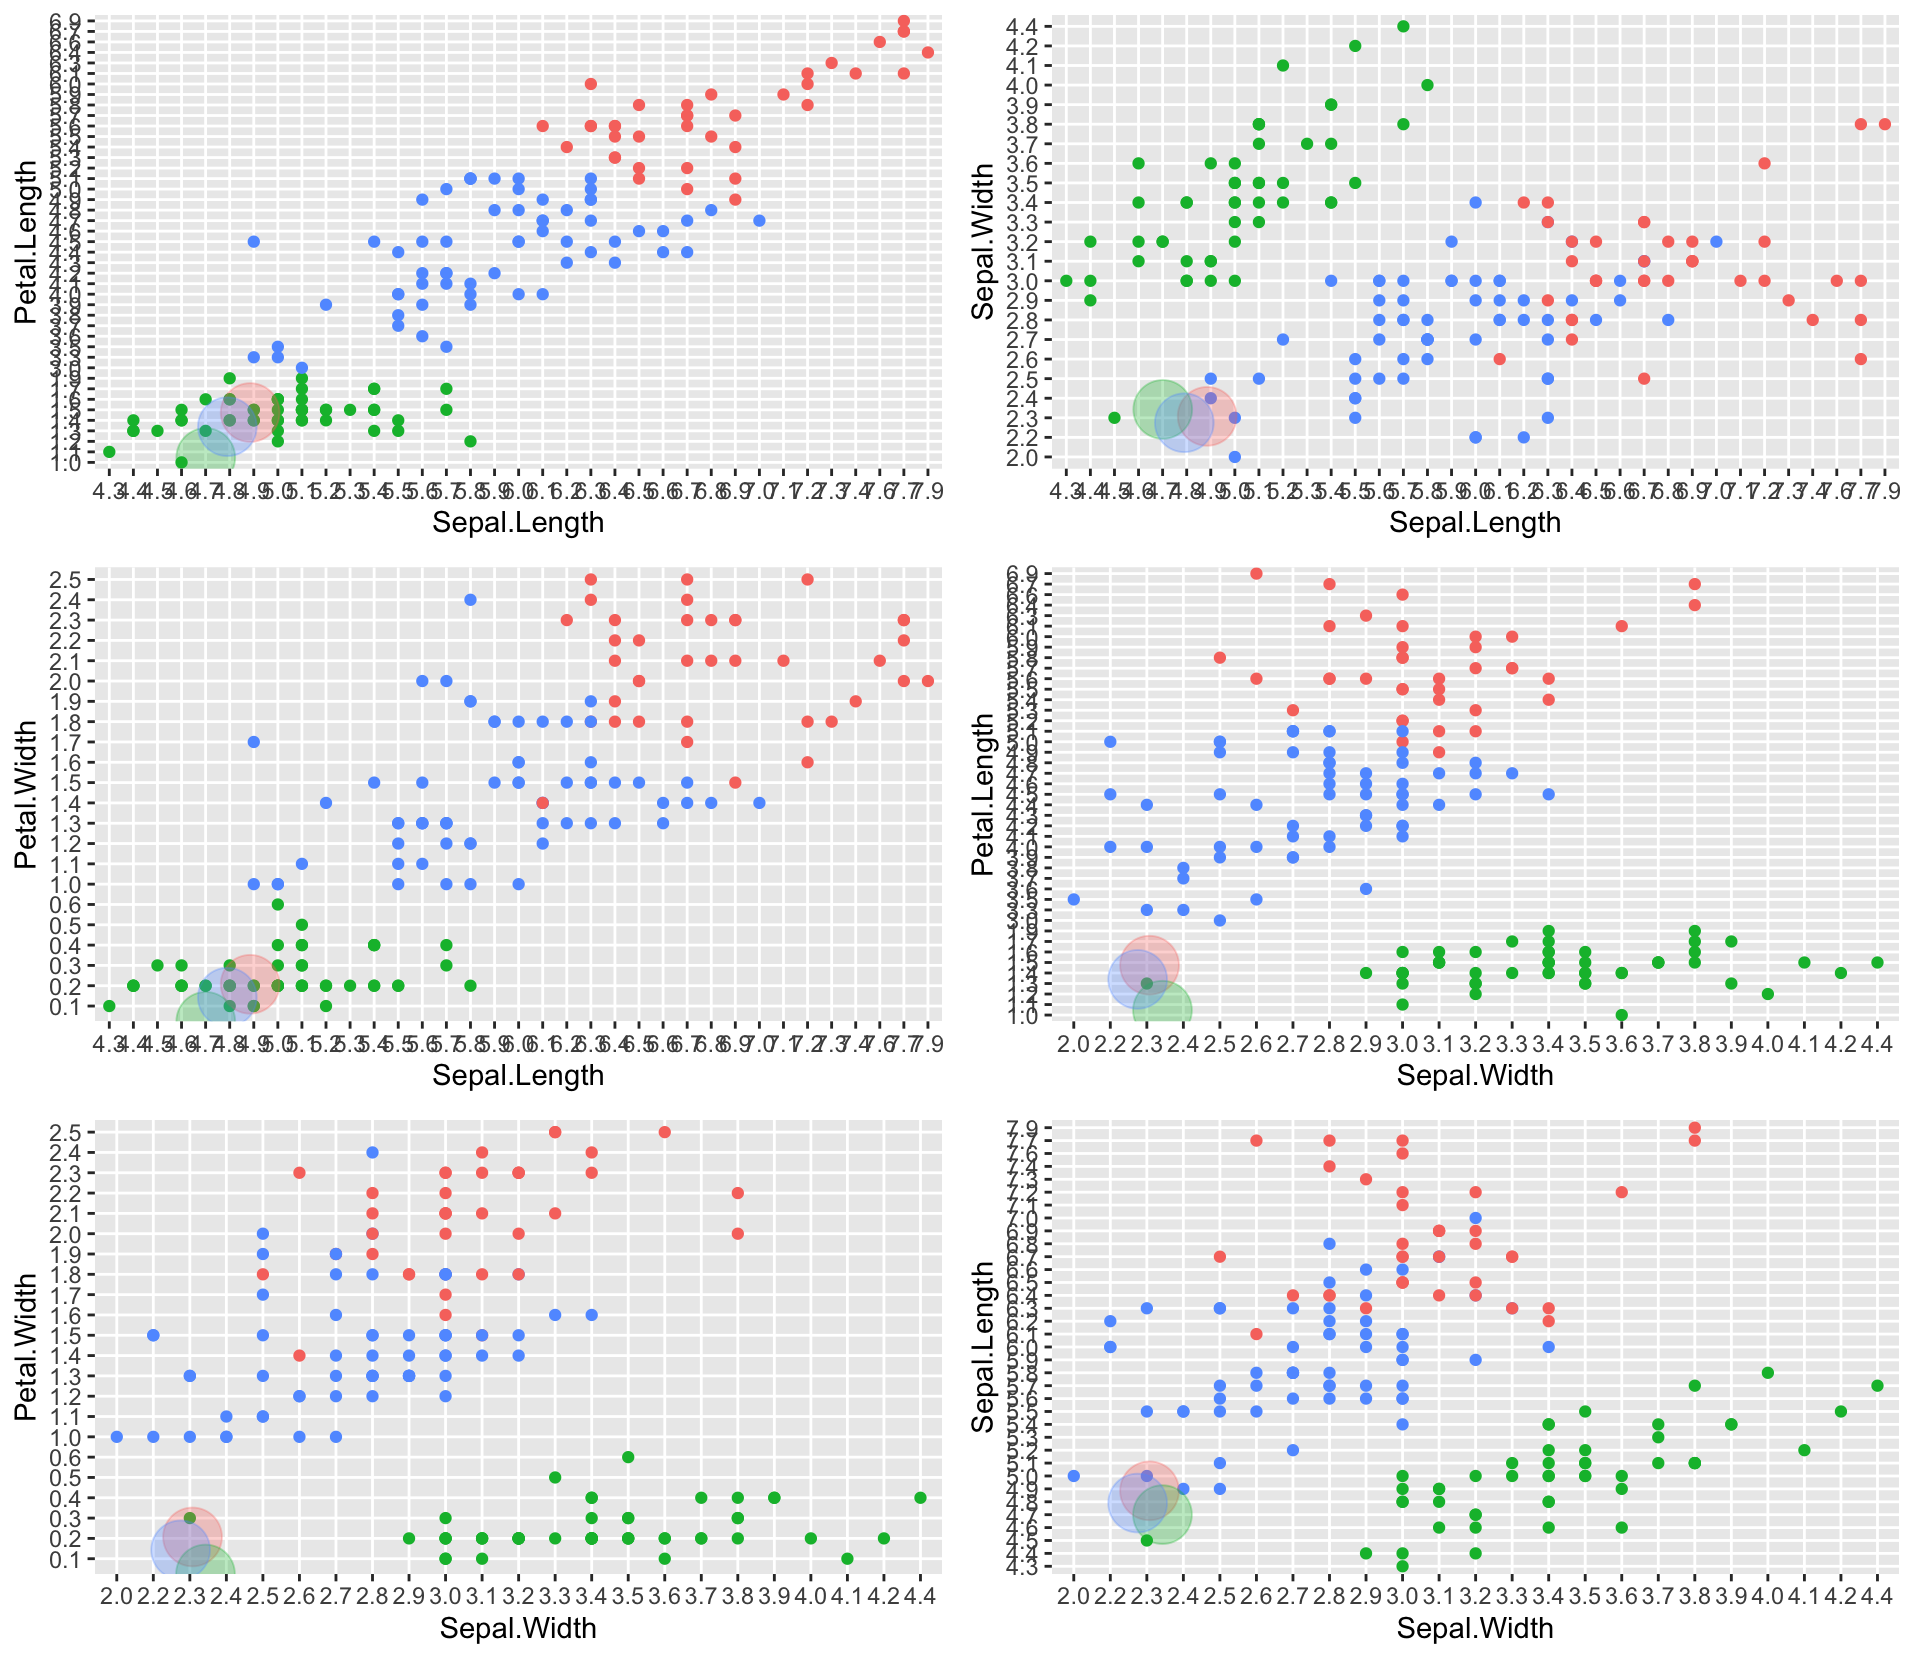
\includegraphics[width=1\textwidth]{Fig5}
\end{figure}

\subsection{Answer 5}
Here we extract 50 data vs 100 data randomly and perform hierarchical agglomerative clustering

\begin{figure}[H]
    \caption{50 data cluster dendrogram}
    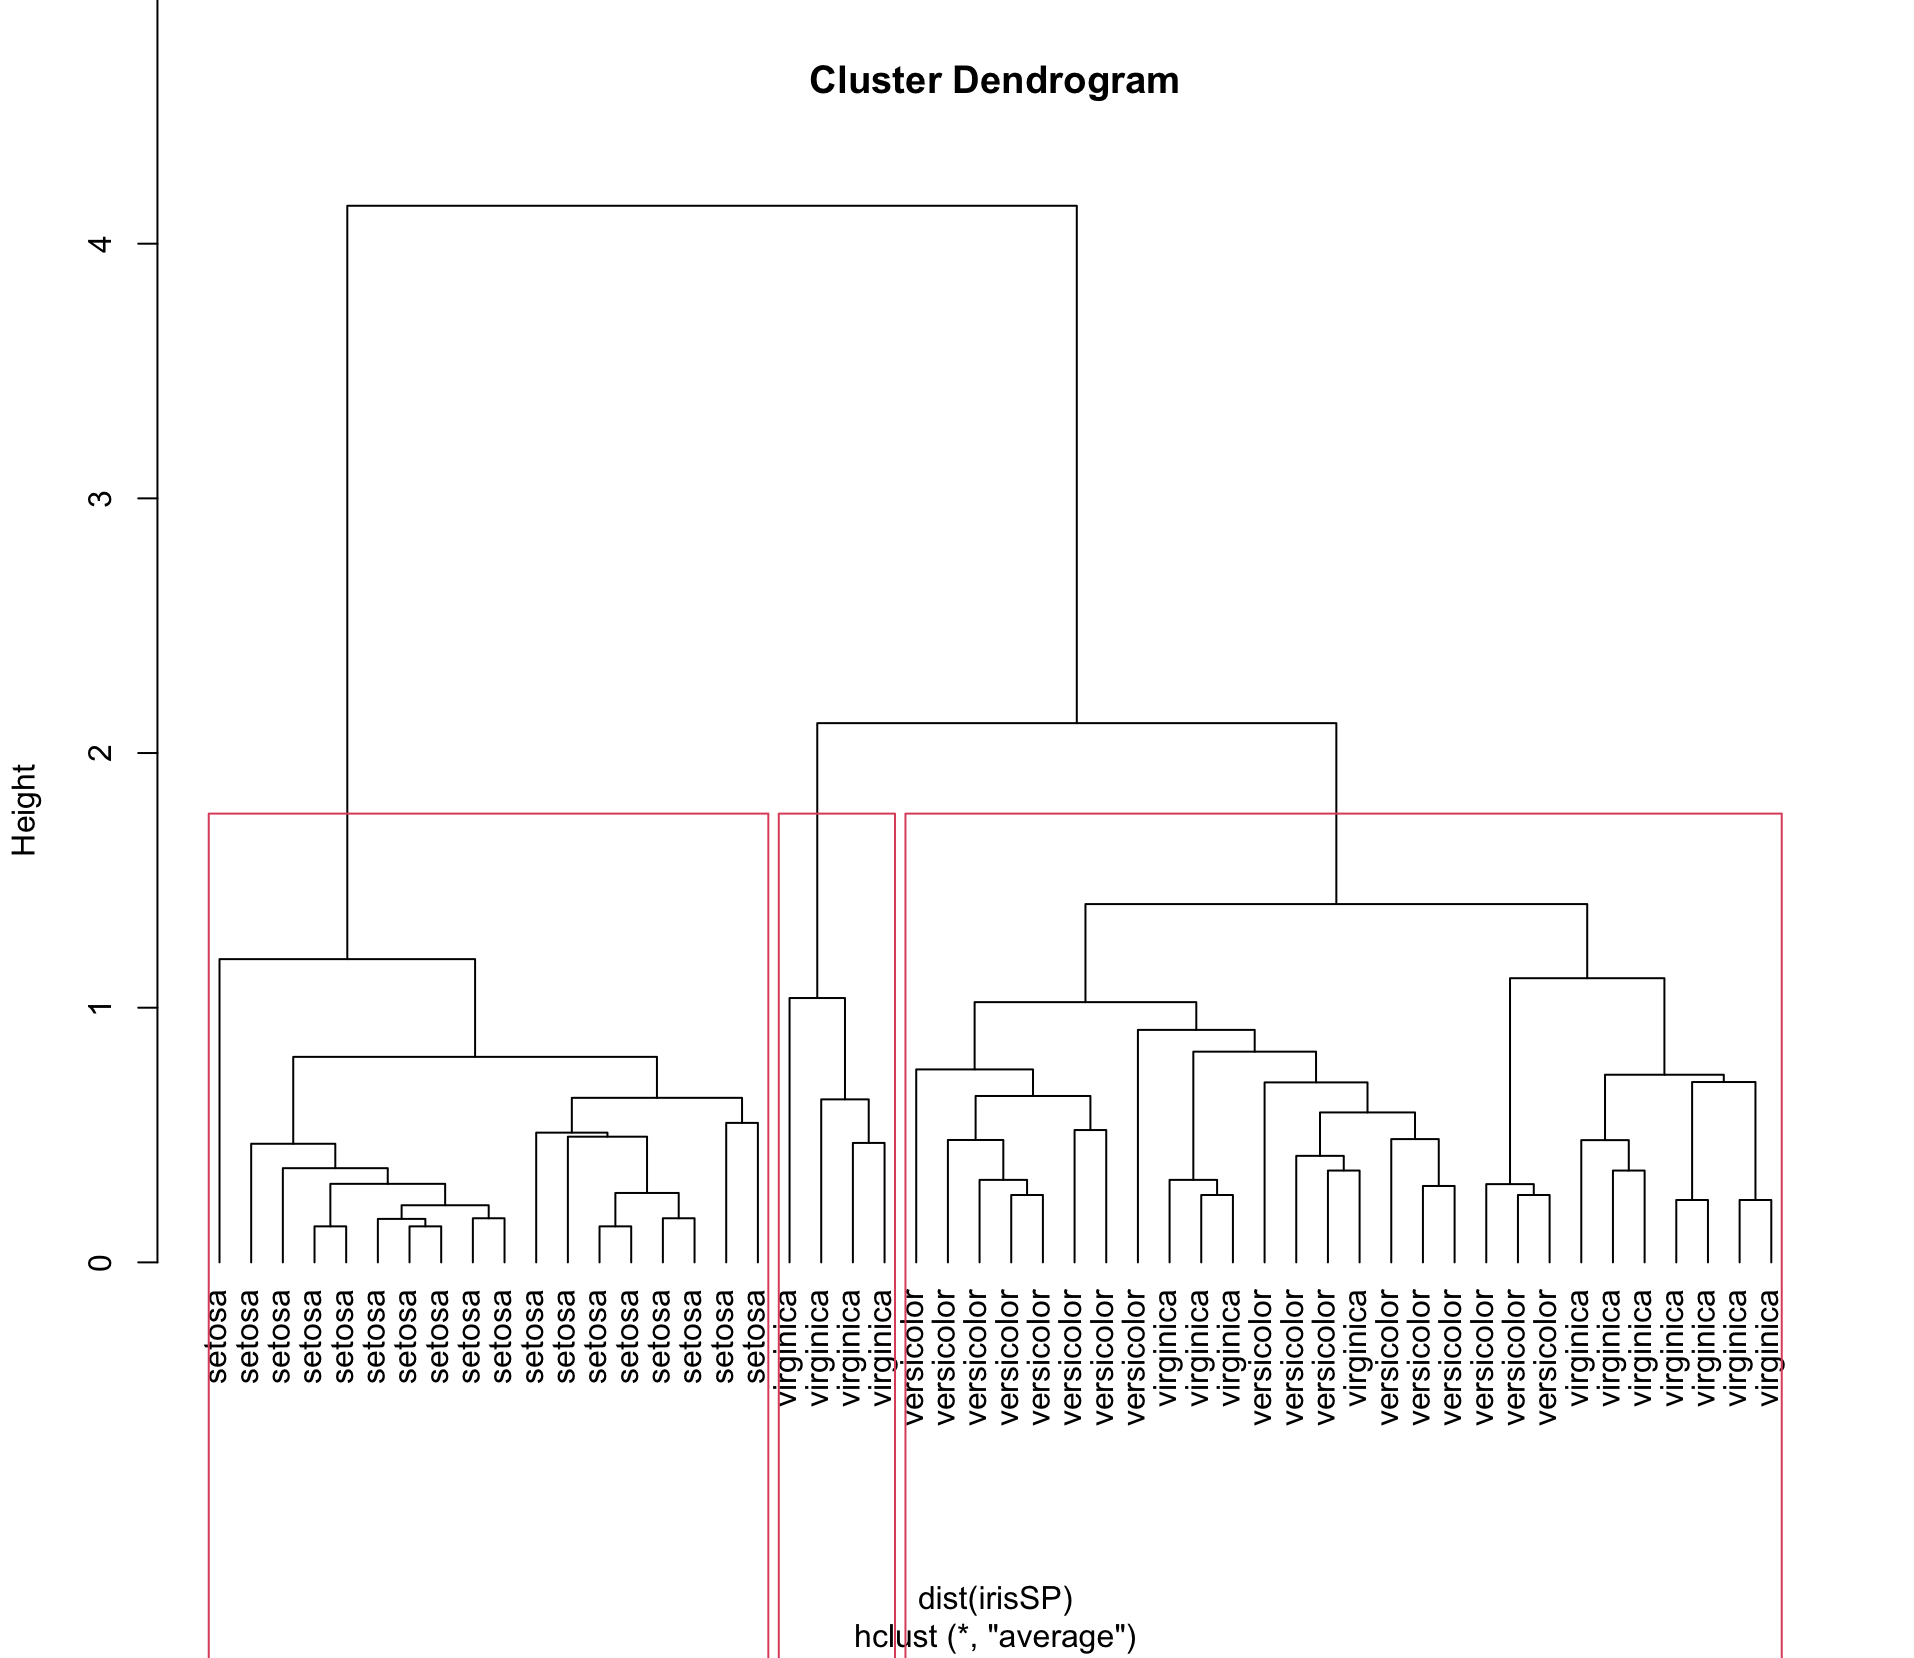
\includegraphics[width=1\textwidth]{Fig6}
\end{figure}

\begin{figure}[H]
    \caption{100 data cluster dendrogram}
    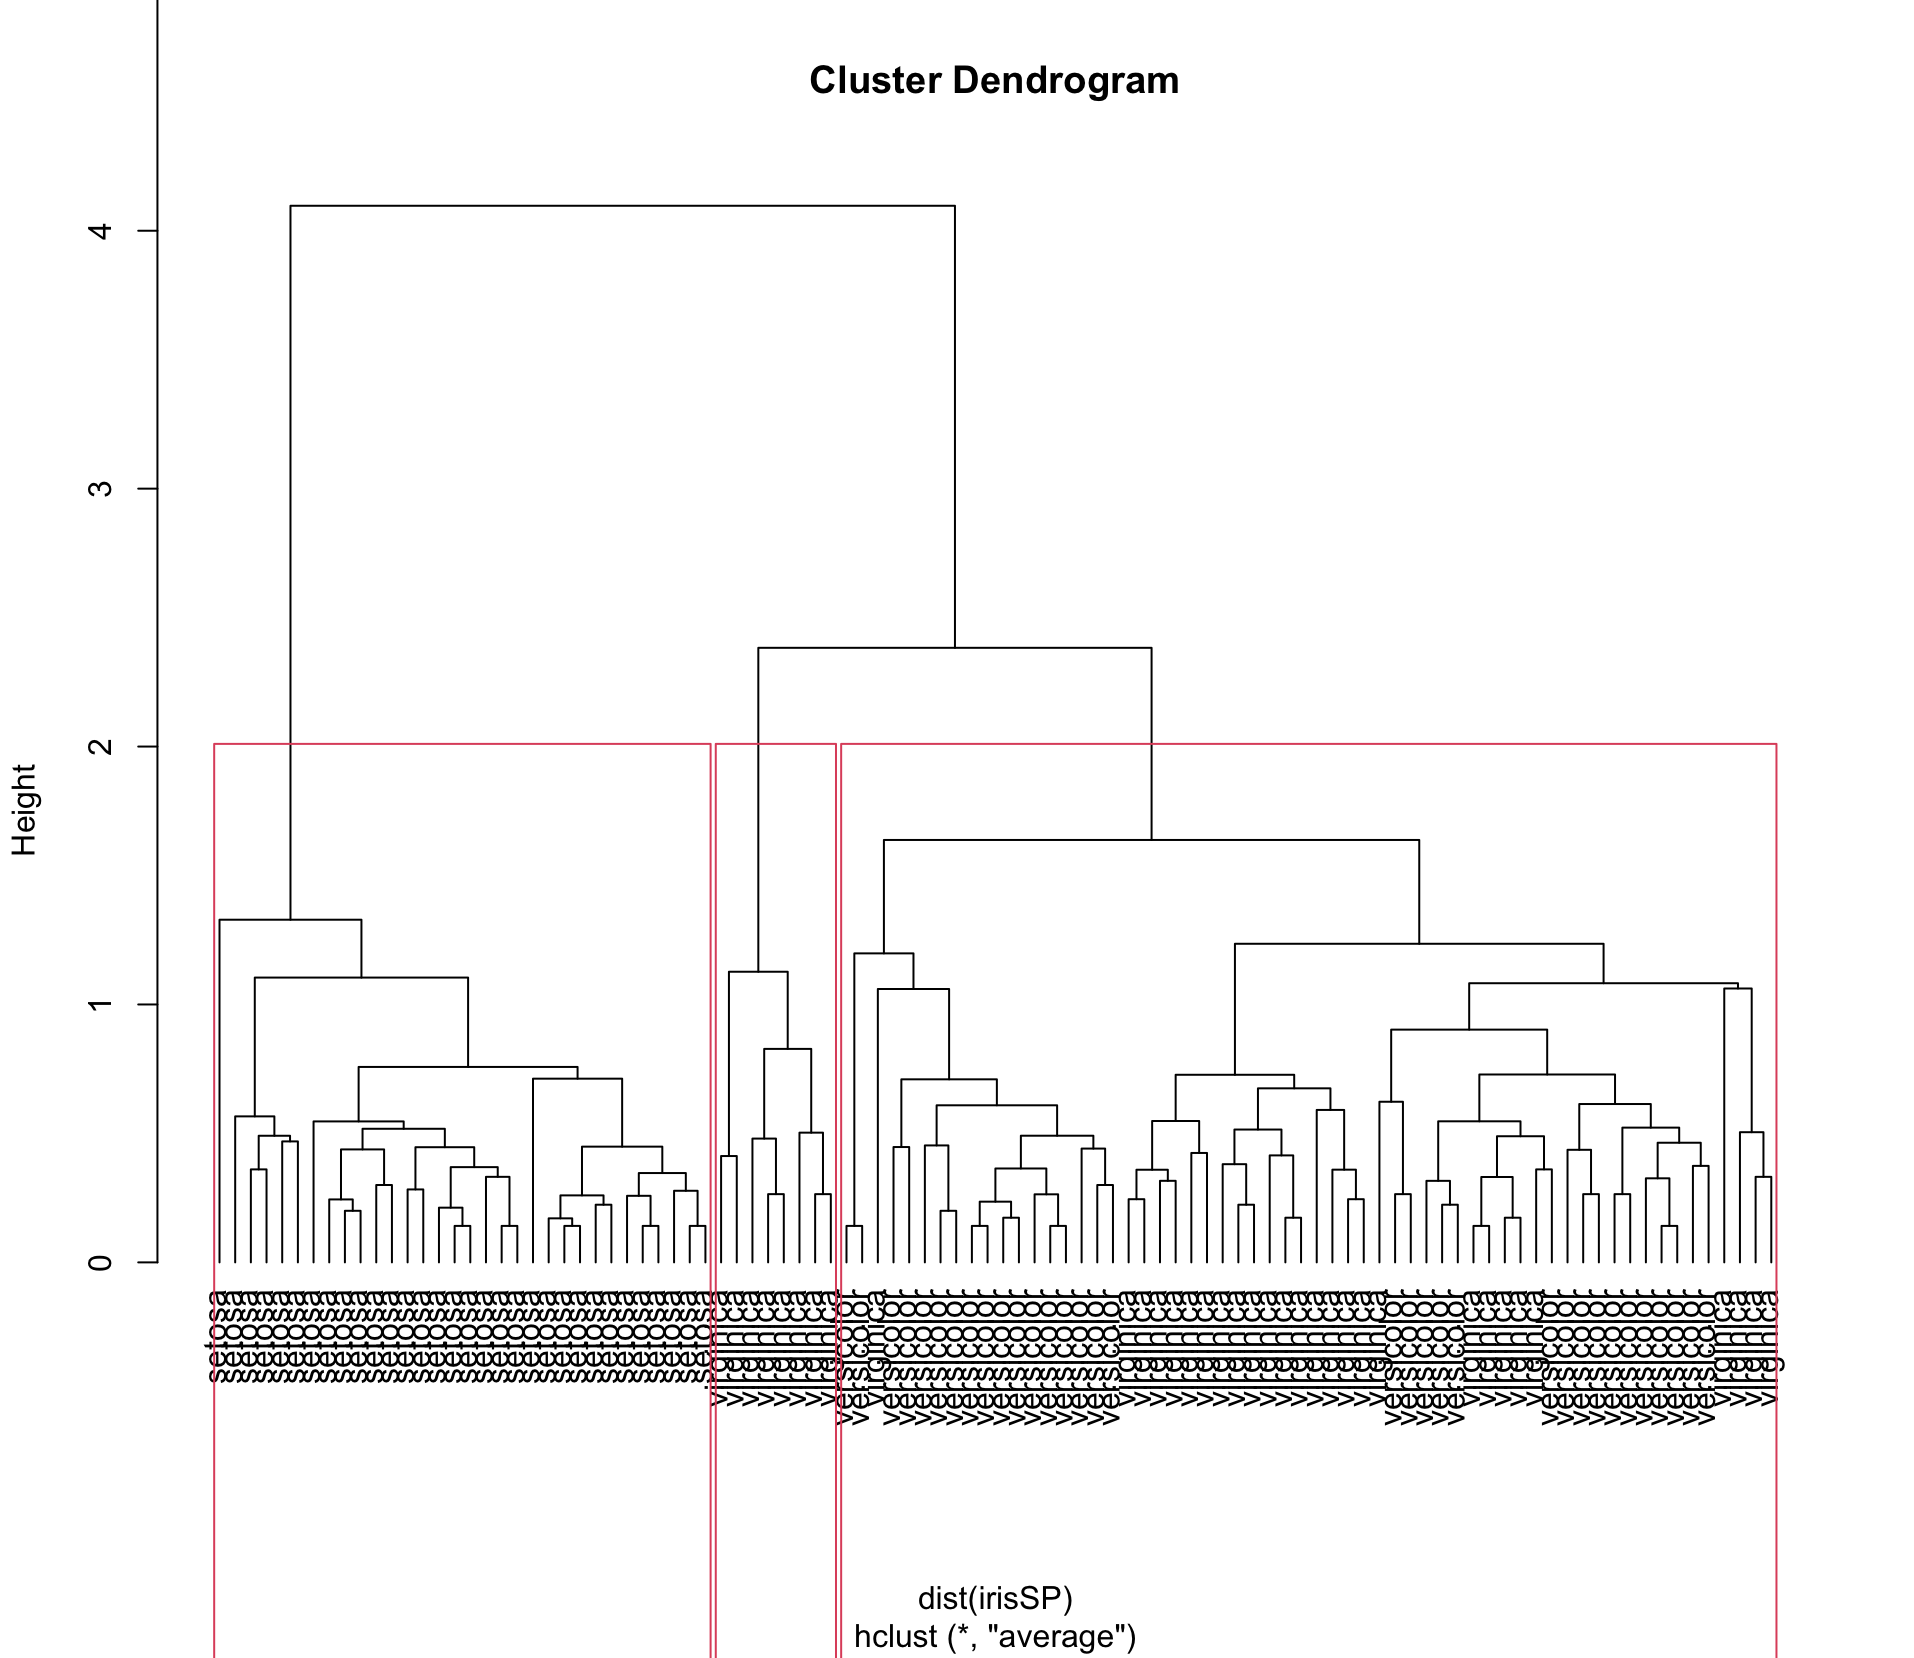
\includegraphics[width=1\textwidth]{Fig7}
\end{figure}


\subsection{Source Code}
\begin{lstlisting}
library(plyr)
#install.packages('ggplot2')
#install.packages('colorspace')
library(ggplot2)
library(cluster)
library(lattice)
library(graphics)
library(grid) 
library(gridExtra)

raw_input = as.data.frame(iris)
kmdata_org = as.matrix(raw_input[,c("Sepal.Length","Sepal.Width","Petal.Length","Petal.Width","Species")])
summary(raw_input)

colors <-c("red","green","blue")
pairs(iris[1:4],pch=21,bg=colors[unclass(iris$Species)])

par(xpd=TRUE)
legend(0.2,0.02,horiz=TRUE,as.vector(unique(iris$Species)),fill=colors,bty="n")

kmdata <- kmdata_org[,1:4]

wss <- numeric(15)
for (k in 1:15) 
  wss[k] <- sum(kmeans(kmdata, centers=k,nstart=25)$withinss)
plot(1:15, wss, type="b", xlab="Number of Clusters", ylab="Within Sum of Squares")

km = kmeans(kmdata, 3)
km
str(km)
table(iris$Species,km$cluster)

df = as.data.frame(kmdata[,1:4])
df$cluster = factor(km$cluster)
centers = as.data.frame(km$centers)

fig1 = ggplot(data=df, aes(x=Sepal.Length, y=Petal.Length, color=cluster ))+geom_point() + geom_point(data=centers,aes(x=Sepal.Length,y=Petal.Length, color=as.factor(c(1,2,3))),size=10, alpha=.3, show.legend = FALSE)
fig2 = ggplot(data=df, aes(x=Sepal.Length, y=Sepal.Width, color=cluster ))+geom_point() + geom_point(data=centers,aes(x=Sepal.Length, y=Sepal.Width, color=as.factor(c(1,2,3))),size=10, alpha=.3, show.legend = FALSE)
fig3 = ggplot(data=df, aes(x=Sepal.Length, y=Petal.Width, color=cluster ))+geom_point() + geom_point(data=centers,aes(x=Sepal.Length,y=Petal.Width, color=as.factor(c(1,2,3))),size=10, alpha=.3, show.legend = FALSE)
fig4 = ggplot(data=df, aes(x=Sepal.Width, y=Petal.Length, color=cluster ))+geom_point() + geom_point(data=centers,aes(x=Sepal.Width,y=Petal.Length, color=as.factor(c(1,2,3))),size=10, alpha=.3, show.legend = FALSE)
fig5 = ggplot(data=df, aes(x=Sepal.Width, y=Petal.Width, color=cluster ))+geom_point() + geom_point(data=centers,aes(x=Sepal.Width,y=Petal.Width, color=as.factor(c(1,2,3))),size=10, alpha=.3, show.legend =  FALSE)
fig6 = ggplot(data=df, aes(x=Sepal.Width, y=Sepal.Length, color=cluster ))+geom_point() + geom_point(data=centers,aes(x=Sepal.Width,y=Sepal.Length, color=as.factor(c(1,2,3))),size=10, alpha=.3, show.legend = FALSE)
grid.arrange(arrangeGrob(fig1 + theme(legend.position = "none"),
                         fig2 + theme(legend.position = "none"),
                         fig3 + theme(legend.position = "none"),
                         fig4 + theme(legend.position = "none"),
                         fig5 + theme(legend.position = "none"),
                         fig6 + theme(legend.position = "none"),
                         ncol = 2))

idx <- sample(1:dim(iris)[1],100)
irisSP <- iris[idx,]
irisSP$Species <- NULL

hc <- hclust(dist(irisSP),method = "ave")
plot(hc, hang= -1, labels = iris$Species[idx])

rect.hclust(hc, k=3)
groups <- cutree(hc, k=3)

\end{lstlisting}


\section{Task 3: Association Rule}

\textbf{Use support 0.01:}
\begin{figure}[H]
    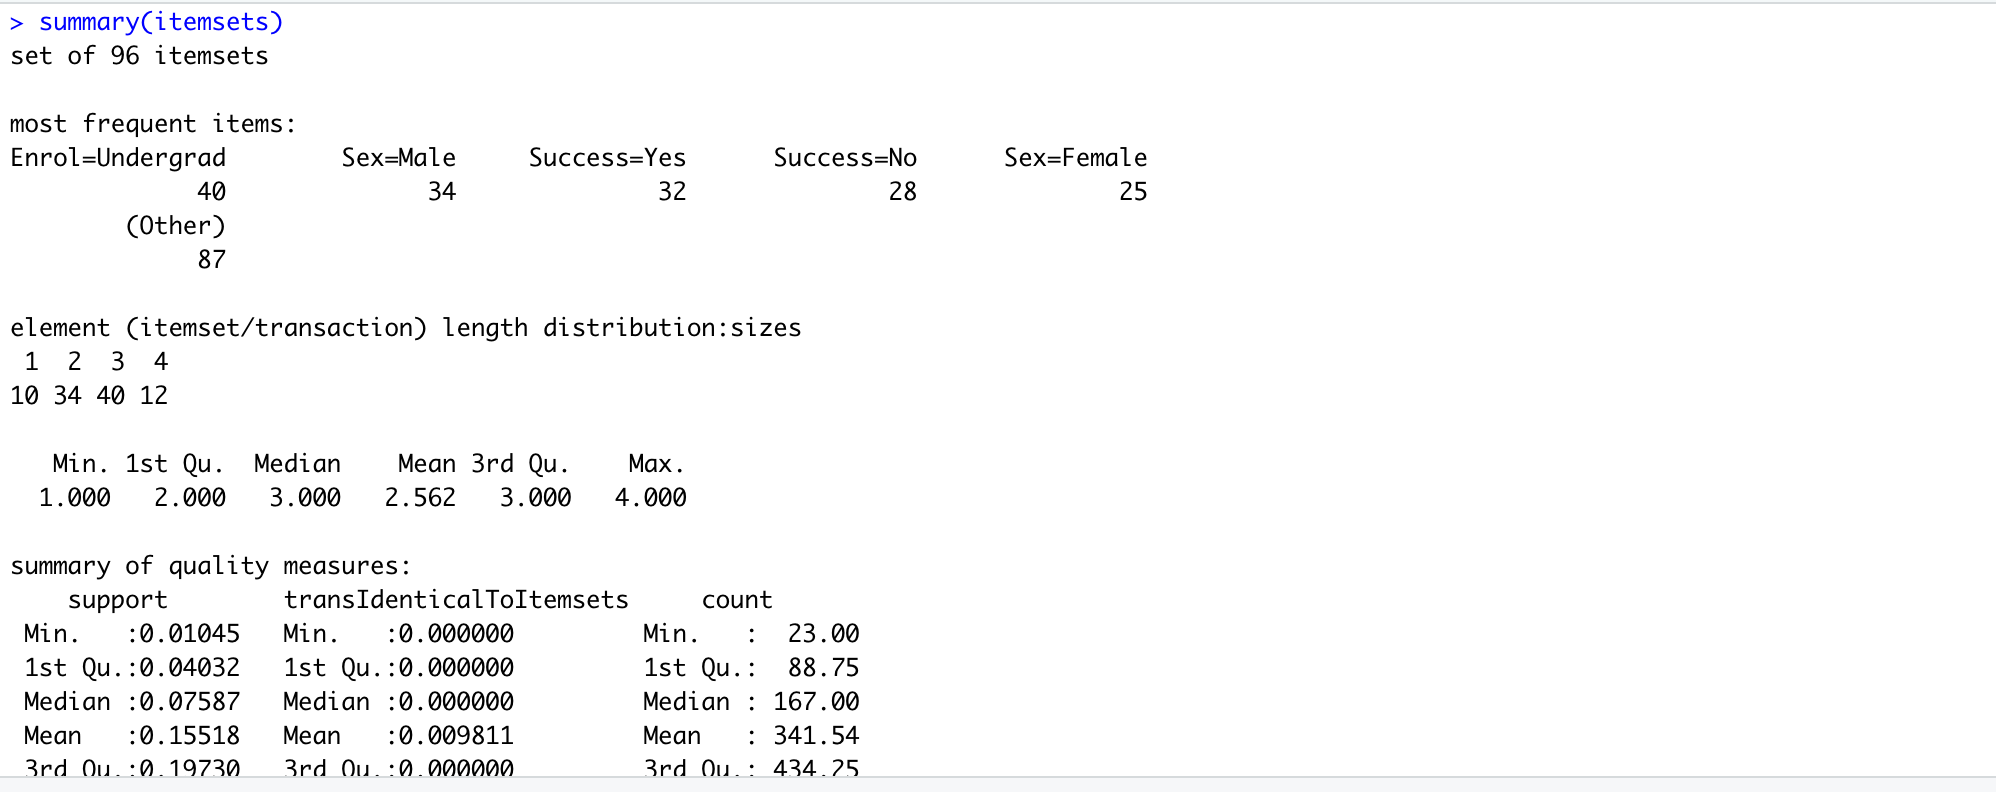
\includegraphics[width=1\textwidth]{Fig8}
\end{figure}

\textbf{Use support 0.02:}
\begin{figure}[H]
    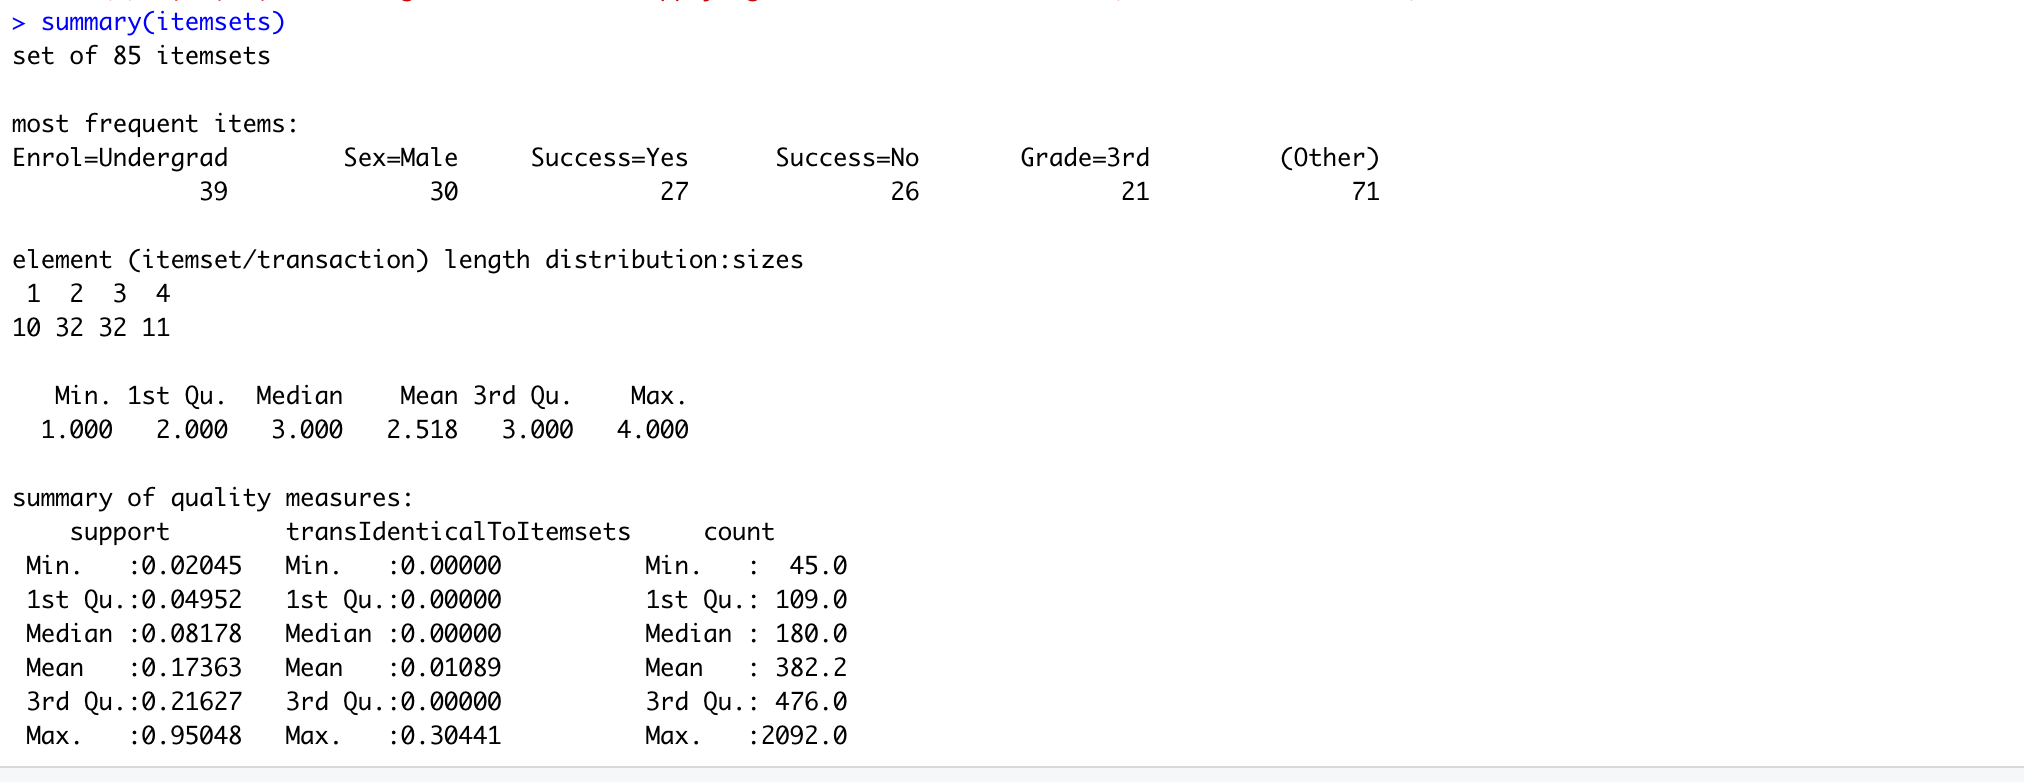
\includegraphics[width=1\textwidth]{Fig9}
\end{figure}


\textbf{Use support 0.05:}
\begin{figure}[H]
    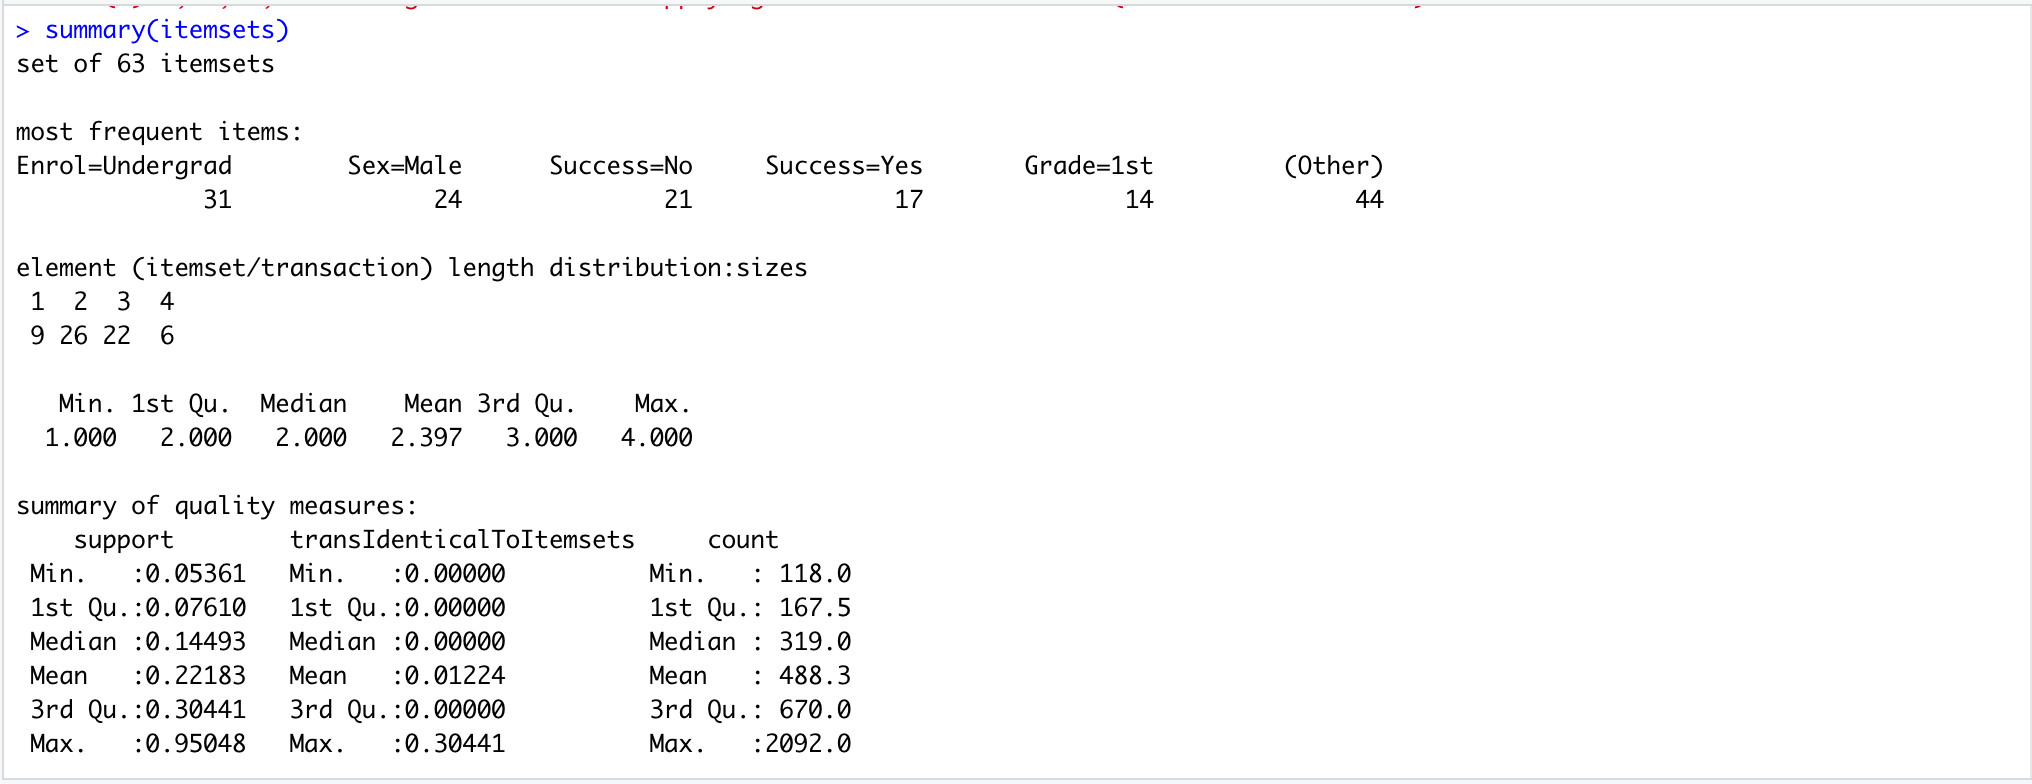
\includegraphics[width=1\textwidth]{Fig10}
\end{figure}

\textbf{Visualization of rules:}
\begin{figure}[H]
    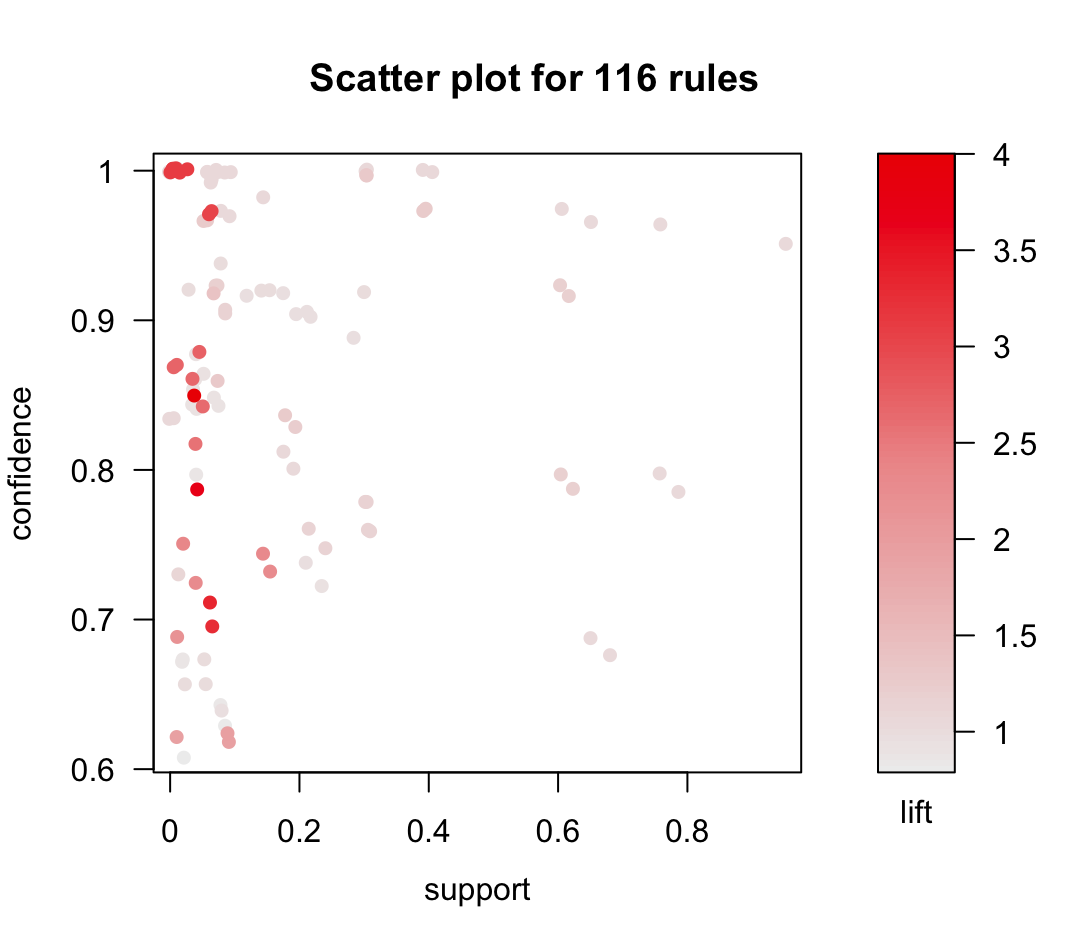
\includegraphics[width=1\textwidth]{Fig11}
\end{figure}

\textbf{Relationship among support, confidence and lift:}
\begin{figure}[H]
    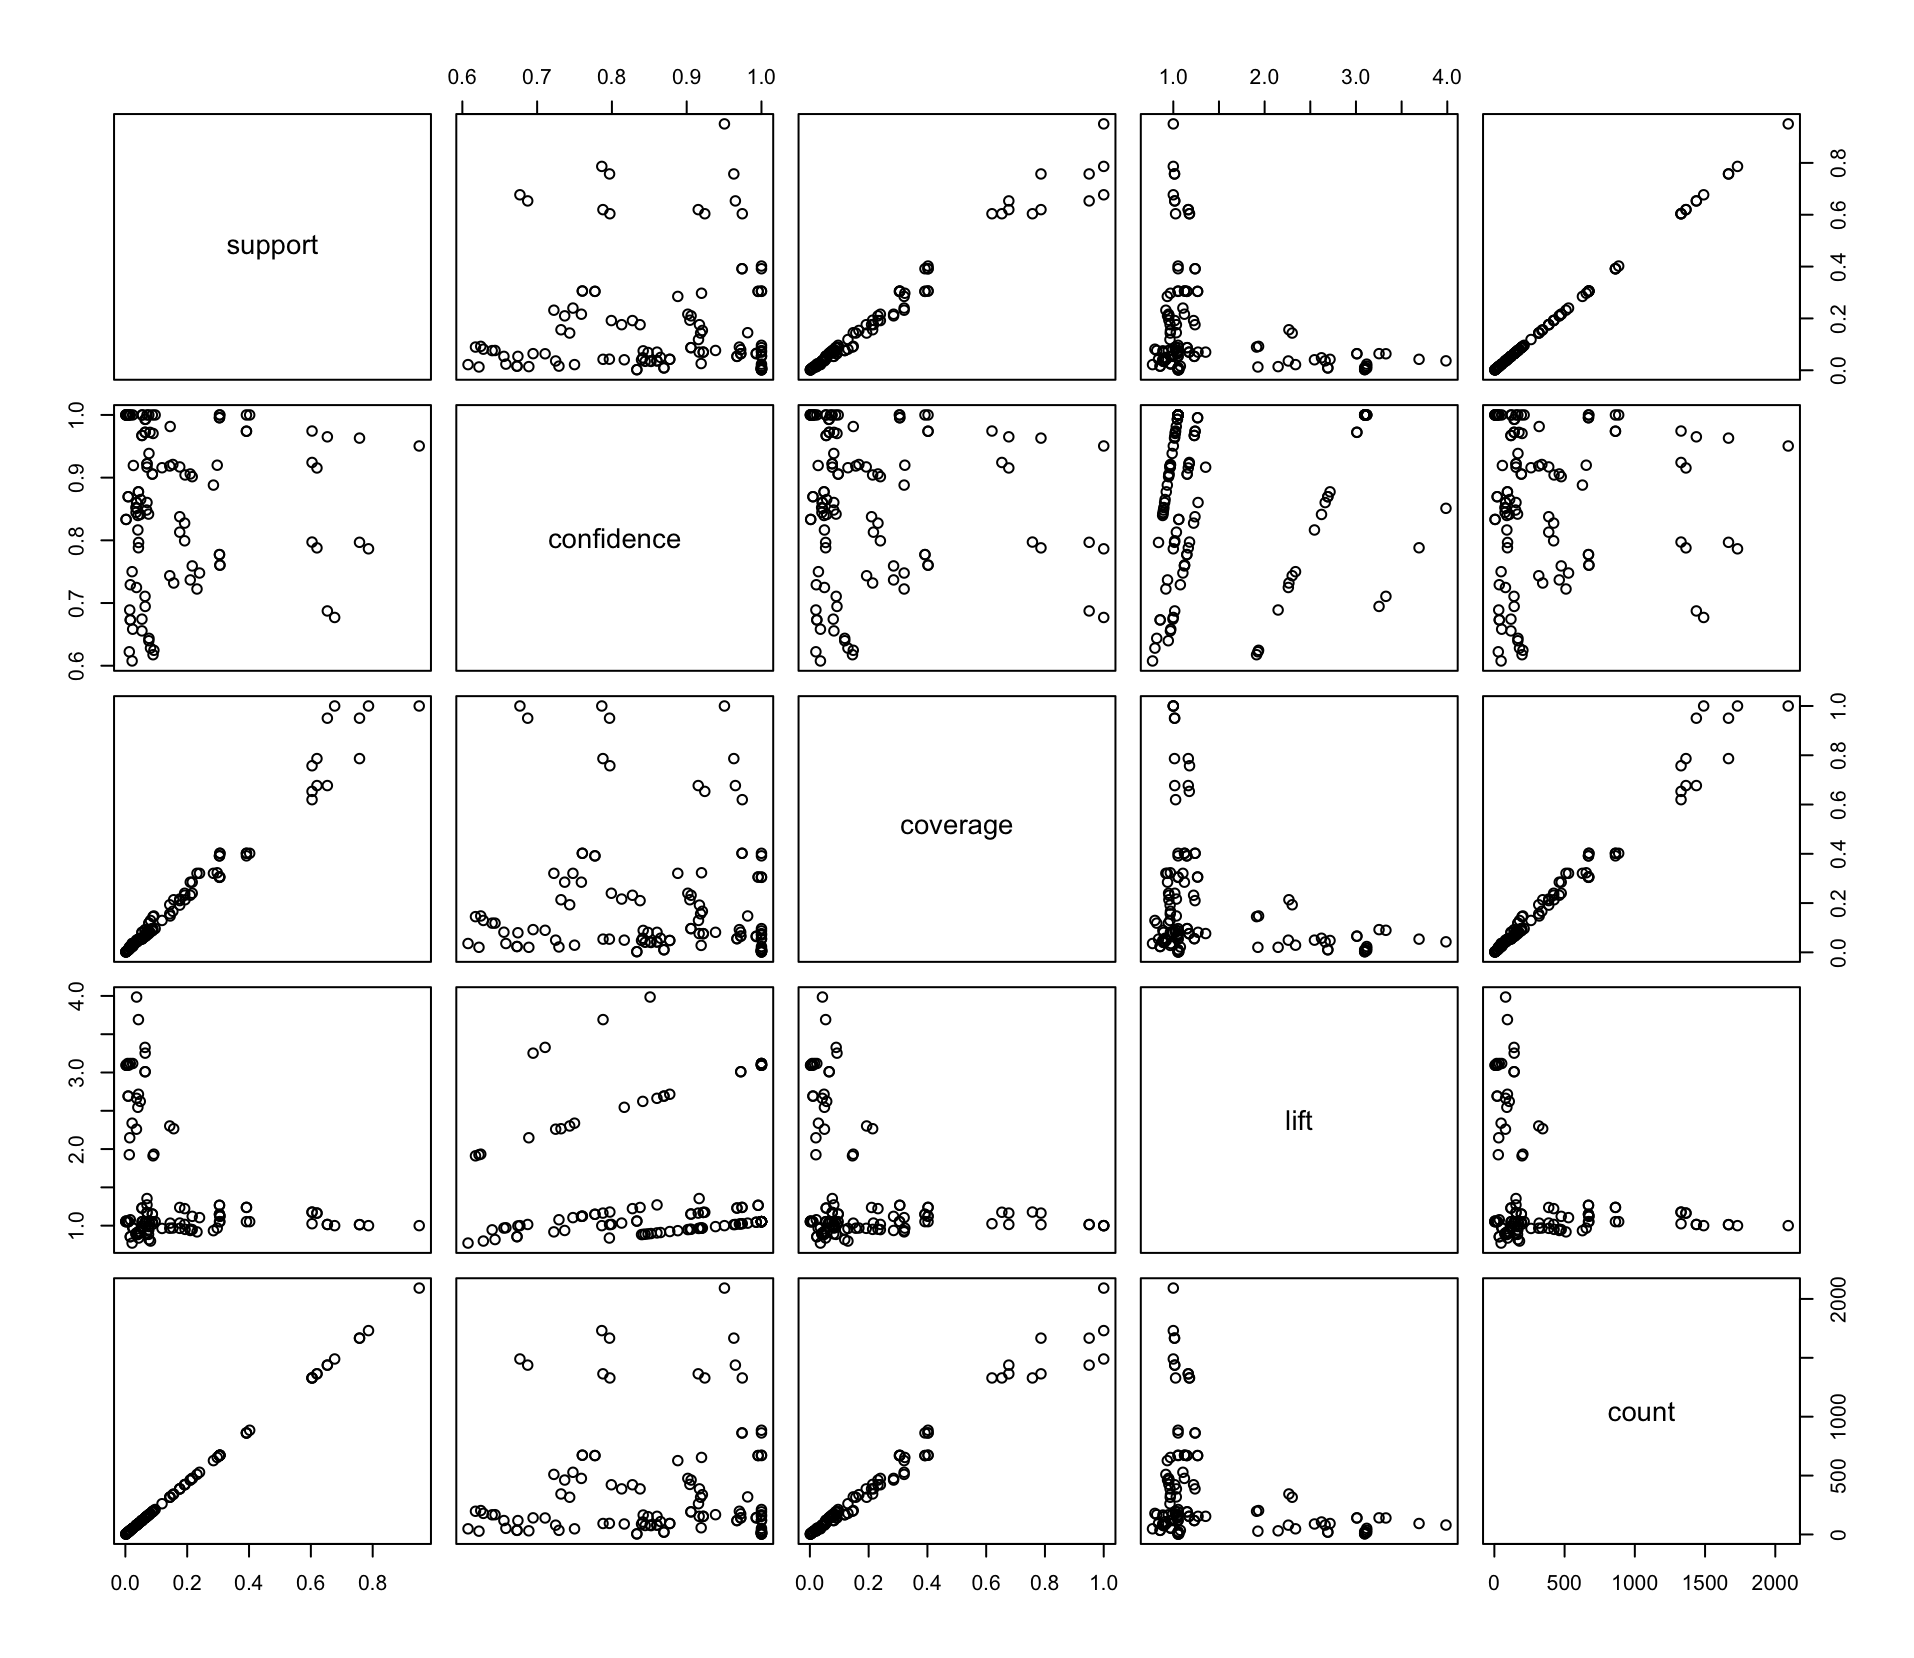
\includegraphics[width=1\textwidth]{Fig12}
\end{figure}

\textbf{Visualization of graphs:}
\begin{figure}[H]
    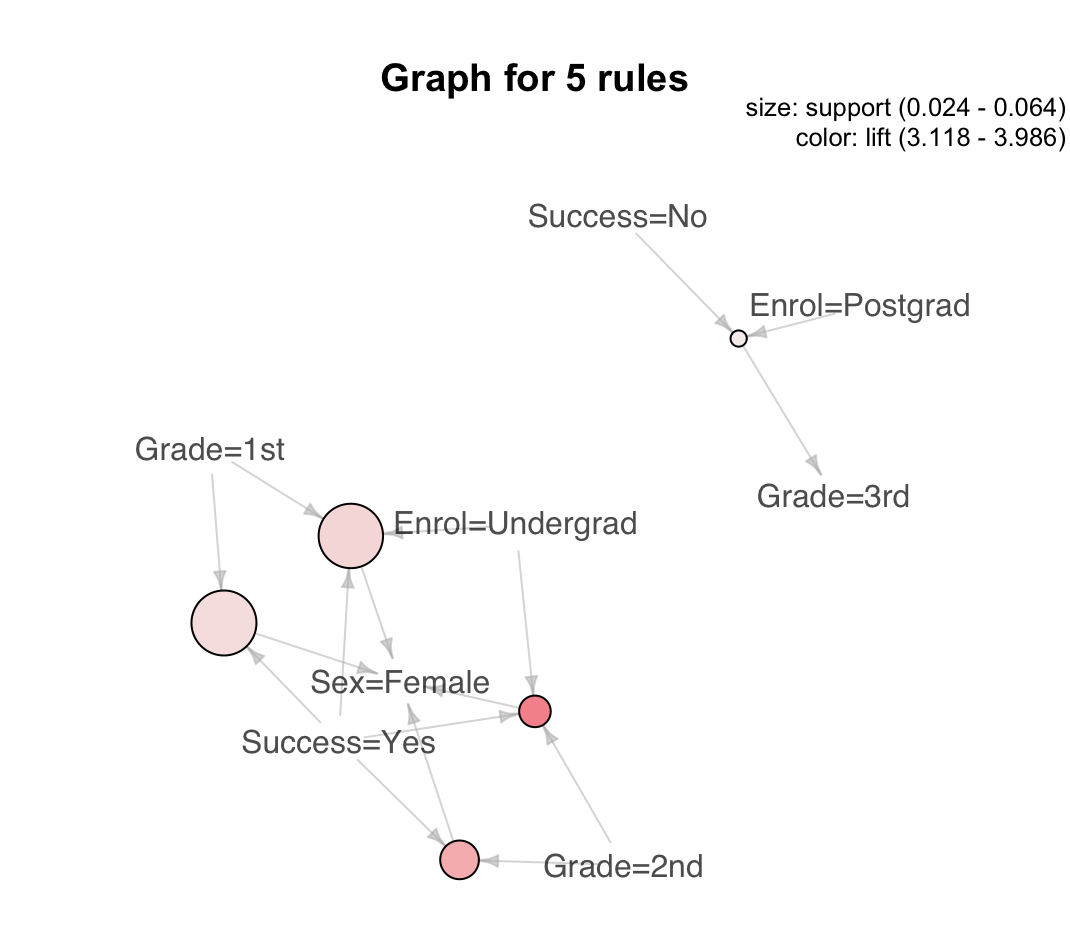
\includegraphics[width=1\textwidth]{Fig13}
\end{figure}

\textbf{Source Code:}
\begin{lstlisting}
library(arules)
library(arulesViz)

df <- read.csv("A1_success_data.csv")

itemsets<- apriori(df, parameter=list(minlen=1, maxlen=10, support=0.01, target="frequent itemsets"))

summary(itemsets)

itemsets<- apriori(df, parameter=list(minlen=1, maxlen=10, support=0.02, target="frequent itemsets"))

summary(itemsets)

itemsets<- apriori(df, parameter=list(minlen=1, maxlen=10, support=0.05, target="frequent itemsets"))

summary(itemsets)


rules<- apriori(df, parameter=list(support=0.001,confidence=0.6, target = "rules"))
plot(rules)
plot(rules@quality)

slope<- sort(round(rules@quality$lift / rules@quality$confidence, 2))
unlist(lapply(split(slope,f=slope),length))
inspect(head(sort(rules, by="lift"), 10))
inspect(head(sort(rules, by="confidence"), 10))
inspect(head(sort(rules, by="support"), 10))

confidentRules<- rules[quality(rules)$confidence > 0.9]
plot(confidentRules, method="matrix", measure=c("lift", "confidence"))

highLiftRules <- head(sort(rules, by="lift"), 5) 
plot(highLiftRules, method="graph", control=list(type="items"))

test<-inspect(sort(rules, by="lift"))
test[test$rhs=="{Success=Yes}",]
test[test$rhs=="{Success=No}",]

\end{lstlisting}
\end{document}
